\chapter{Model}
To make the quadcopter airborn and have a steady flight mode it is necessary to derive a model of the system, that describes it's physical behaviour. From this a control system must be designed such that the desired characteristics for the flying is obtained. 
This chapter presents the model. 

First a model overview is presented, then the model deriviation and lastly the model is linearized, as this is necesarry to be able to design a control system. The model and the linearized model is compared by simulations to ensure, that the linear model is an acceptable model approximation.

\section{Model overview}
The model can be split into two sub models. One being an angular model, describing how the angles influence each other in pitch, roll and yaw. The other sub model is a translational velocity model, that describes the velocities in the directions of the x-, y- and z-axis. 
These models will later be combined. 
\begin{figure}[H]
\centering
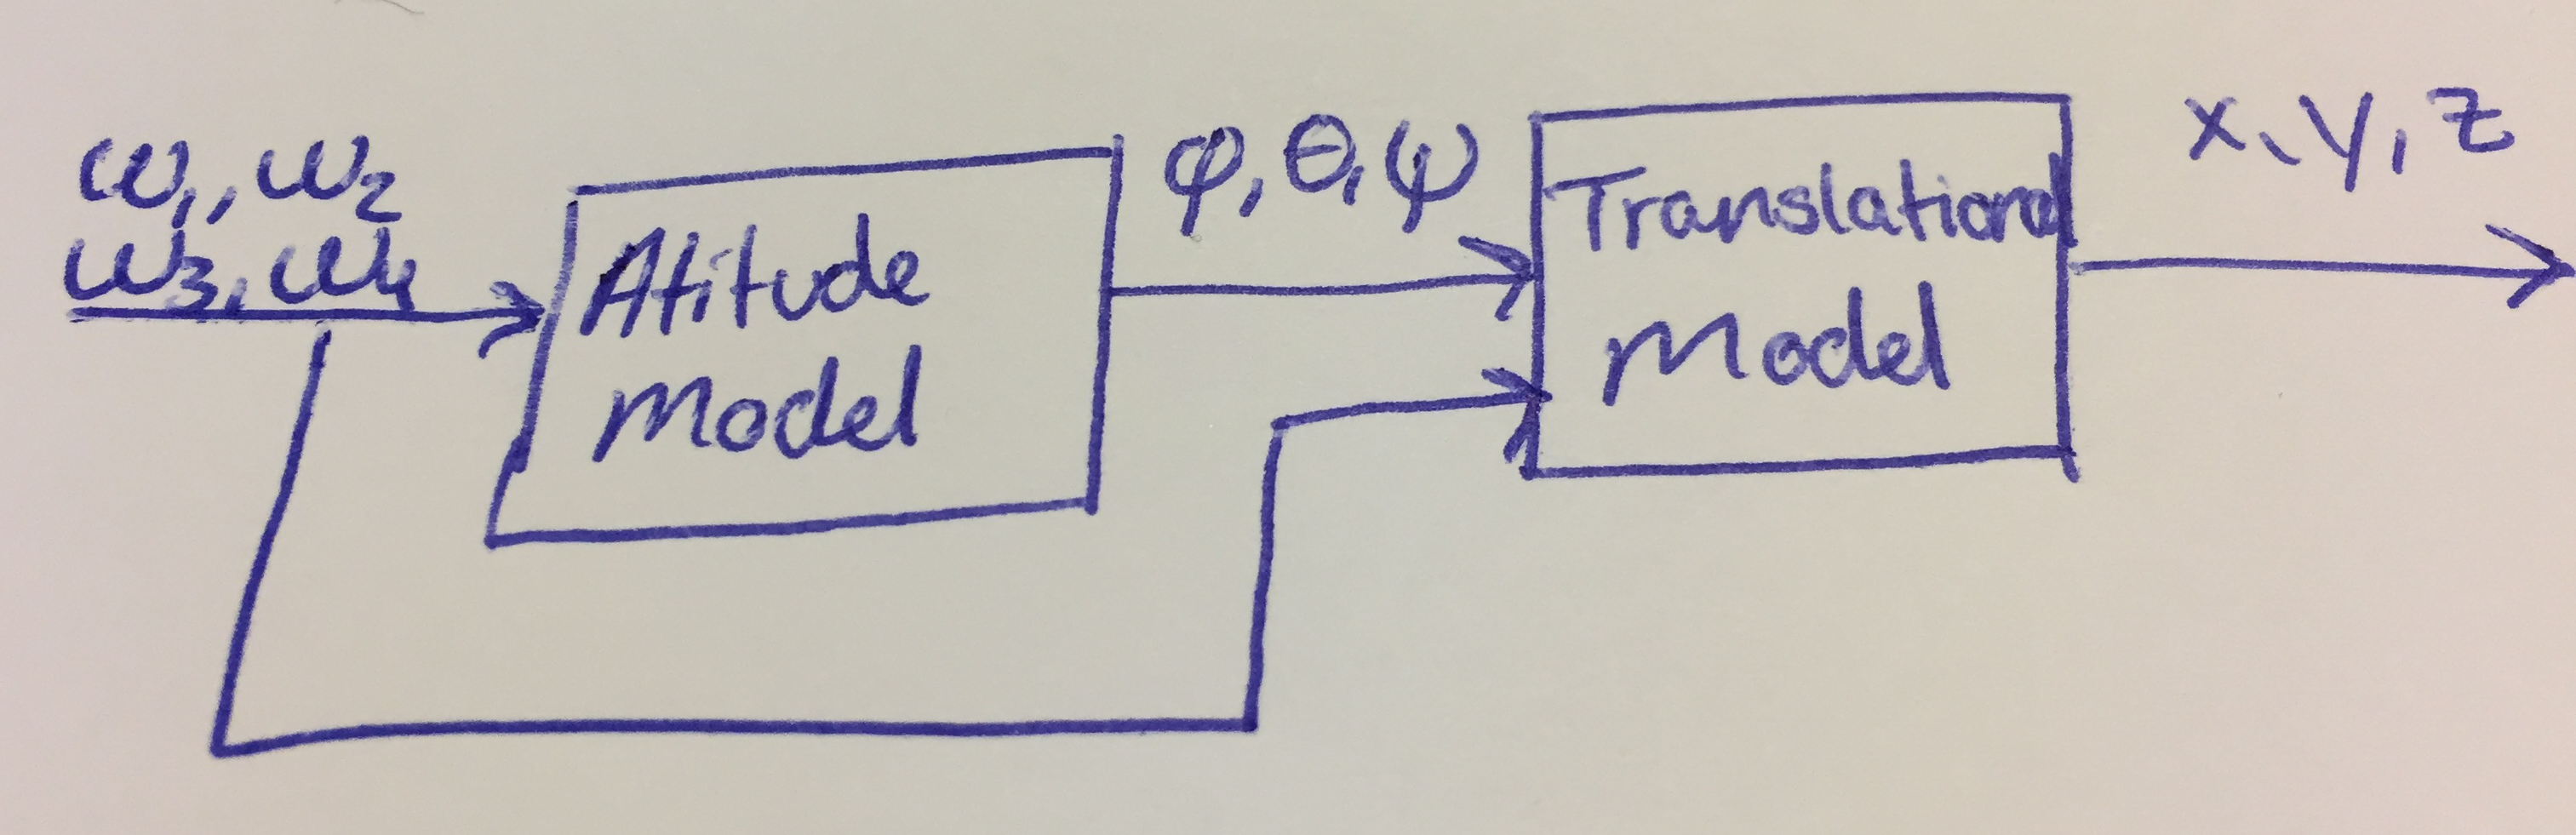
\includegraphics[scale=0.1]{figures/modeloverview.PNG}
\caption{Overview of how the model is split.}
\label{sss}
\end{figure}
When modelling the quadcopter, two coordinate systems are used. A body frame, that is a coordinate system, that is fixed to the flying object and an initial frame, that is a coordinate system that is fixed as the Vicon room. 

It is necessary to use both, as it is desired to know where the quadcopter is within the initial frame to determine its position. To obtain the orientation of the quadcopter, the body frame's orientation compared to the initial frame yields the angles of pitch, roll and yaw. 

 

%Angle and Linear
%Explain the two frames and include drawing showing them
%Flow of the chapter

%\Figref{diagramQuad} shows a representation of the quadcopter where two reference systems, inertial and body, can be seen, as well as the conventions for angles of rotation and forces. \Figref{diagramTorque} shows the body from above and includes the chosen convention for the torques produced by the propellers.
%
%\begin{minipage}{\linewidth}
%	\begin{minipage}{0.45\linewidth}
%		\begin{figure}[H]
%			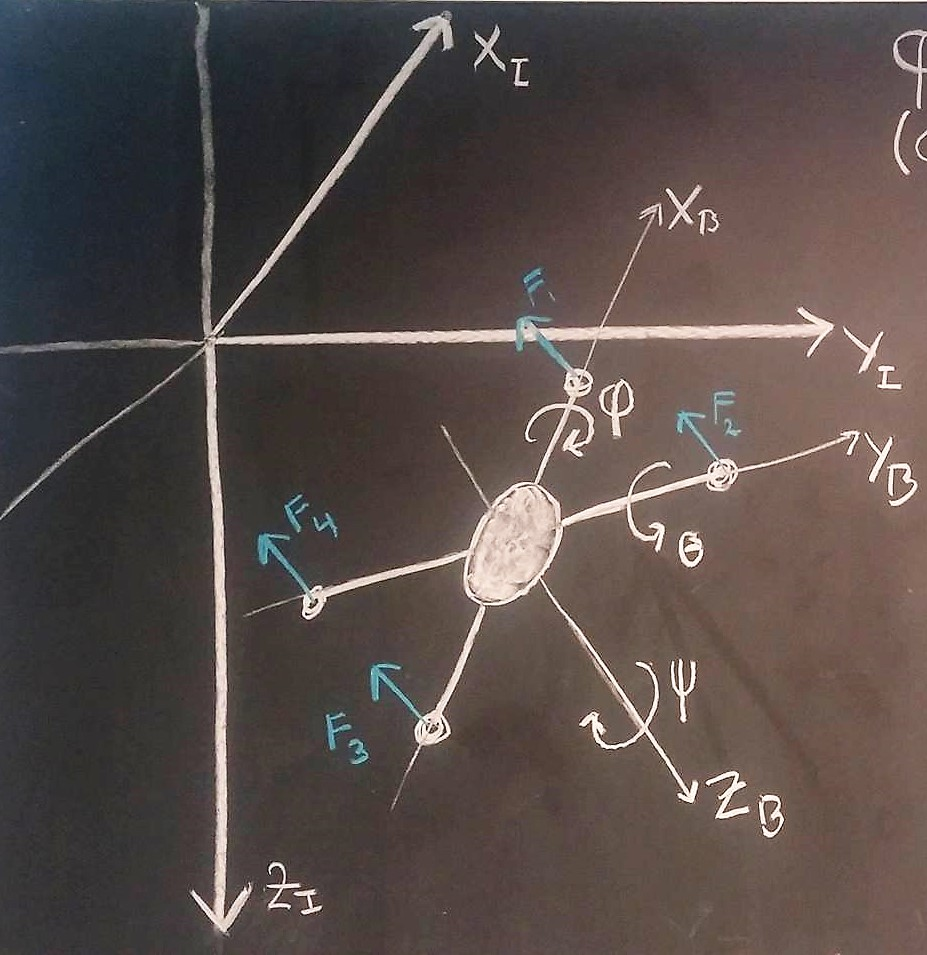
\includegraphics[scale=.27]{figures/drone_diagram}
%			\centering
%			\captionsetup{justification=centering}
%			\captionof{figure}{Diagram of the quadcopter which includes inertial and body reference systems, as well as the references for the angles (roll, pitch and yaw) and the thrust forces produced by the propeller. }
%			\label{diagramQuad}
%		\end{figure}
%	\end{minipage}
%	\hspace{0.03\linewidth}
%	\begin{minipage}{0.45\linewidth}
%		\begin{figure}[H] \vspace{16mm}
%			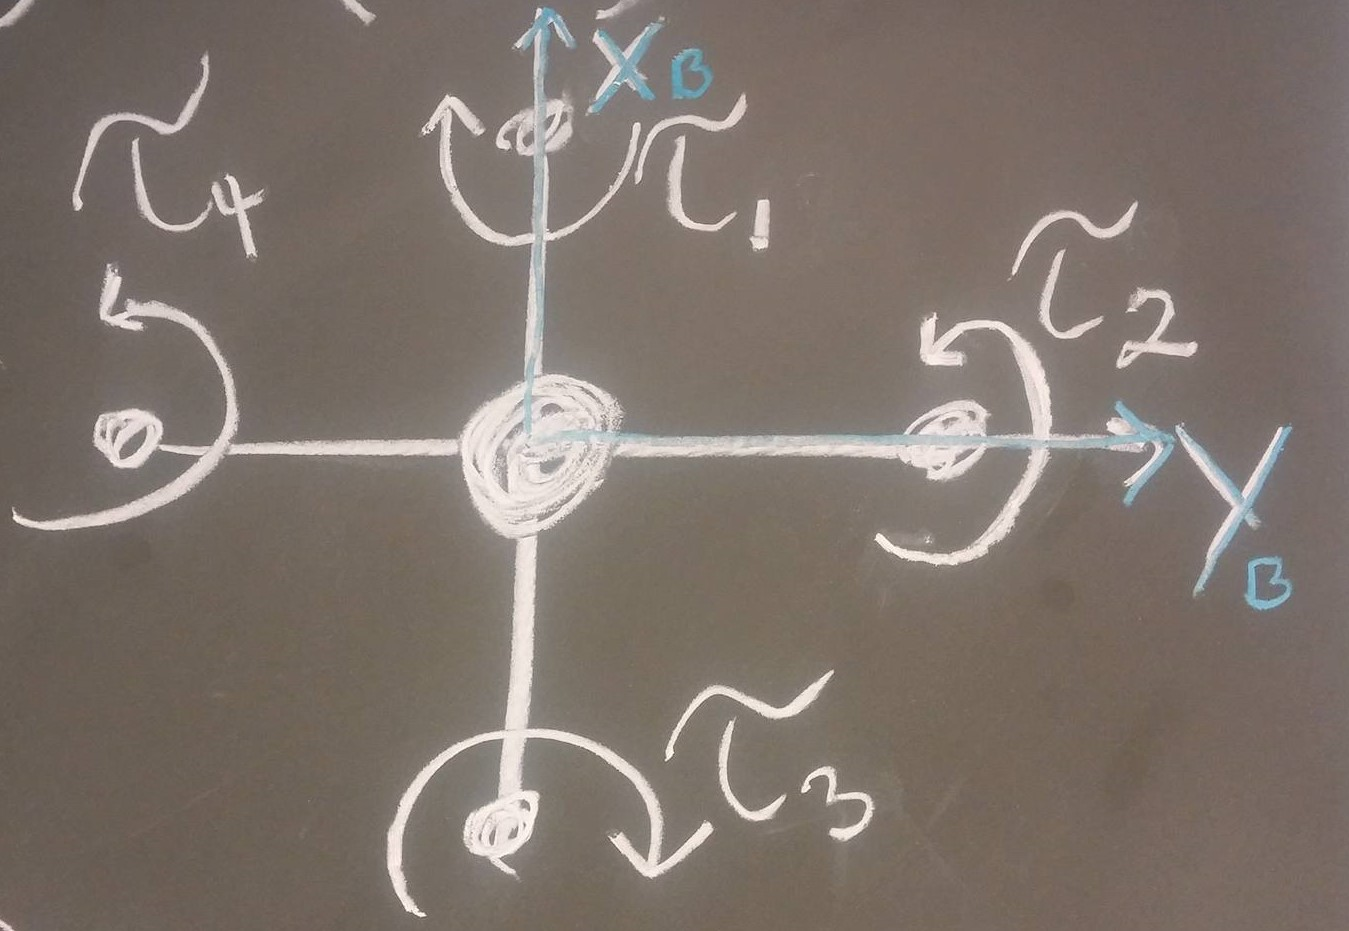
\includegraphics[scale=.18]{figures/torques_diagram}
%			\centering
%			\captionsetup{justification=centering}
%			\captionof{figure}{Diagram of the quadcopter from above, with the references for the torques produced by the drag force at the propeller.}
%			\label{diagramTorque}
%		\end{figure}
%	\end{minipage}
%\end{minipage}
In the following section the attitude model is derived. 